\chapter{Targeted Estimators}
\label{ch-targeted-est}

This chapter is based on Refs.\cite{tlride} and  \cite{hoff}.

The goal of Targeted Estimator (TE) theory is
to find, given an estimator,
a new estimator that is slightly
displaced from the original,
but has better behavior (i.e.,
it converges faster, and with smaller
variance, as the number $N$
of samples grows). This goal and
the strategy one uses to achieve it, is
explained more precisely in the next section.




\section{Goal, Strategy, and Rationale of TE theory}


Let $\rvb = (\rvb_1, \rvb_2, \ldots, \rvb_{n})$ denote
the $n$ nodes of a Bayesian Network, and let $P_\rvb(b)$ for $b\in S_\rvb$
denote the full probability distribution of the bnet.

 Consider a population of
 individuals $\s\in \Sigma$ with $N=|\Sigma|$.
 The {\bf empirical probability distribution}
 $P_N:S_\rvb \rarrow [0,1]$ for this bnet is defined by

\beq
P_N(b) = \frac{1}{N}\sum_\s\delta(b, b^\s)
\eeq

\beq
\sum_b P_N(b)f(b)=
\frac{1}{N}\sum_\s f(b^\s)
\eeq
As $N\rarrow \infty$, $P_N(b)$ tends
to the probability distribution $P_\rvb(b)$
of the bnet.
\begin{figure}[h!]
$$
\xymatrix{
&\rvw_2\ar[ddl]\ar[ddr]
\\
\ul{\xi}_1\ar[r]
&\rvw_1\ar[dr]
&\ul{\xi}_2
\\
\rvd\ar[rr]\ar[u]\ar[rru]
&
&\rvy\ar[u]
}
$$
\caption{Example of bnet considered in TE
theory.}
\label{fig-targeted-bnet}
\end{figure}

Let $\rvb=(\rvX, \ul{\xi})$ and
$\rvX=(\rvd, \rvy,\rvw)$,
where
node $\rvd\in\bool$ denotes a decision to treat a patient,
node $\rvy\in \bool$ denotes the treatment outcome,
multi-node $\rvw$ denotes the covariates
that are good controls, and multi-node $\ul{\xi}$ denotes
the covariates that we don't want to control.
See Fig.\ref{fig-targeted-bnet}
for an example of a bnet that fits this description.


The {\bf estimand} $\haty$ of $y$
is a function $\haty:S_\rvy\times S_\rvw\rarrow \RR$
that minimizes the {\bf loss function} $\call$
given by


\beq
\call[P, \haty]= \sum_X P(X) [y-\haty(x,w)]^2
\;.
\eeq

The {\bf estimator}
 $\Psi[P, \haty]$ for the estimand $\haty$
is defined by

\beq
\Psi[P, \haty] =\sum_X P(X)\haty(d,w)
\eeq

Let
\beq
\delta P(X)=
P(X)-P_{in}(X)
\eeq
where $P, P_{in}:S_\rvX\rarrow [0,1]$ are
probability distributions.

Define $\delta\haty(X)$ by

\beq
\delta\haty(X)= \frac{\haty(d,w) \delta P(X)}{P(X)}
\eeq
Hence

\beq
P(X)\delta\haty(X) = \haty(d,w)\delta P(X)
\eeq
Since $\Psi[P, \haty]$
is linear in $P$ and $\haty$,
it follows that

\beq
\Psi[P, \haty + \delta\haty]=
\Psi[P + \delta P, \haty]
\eeq


Suppose $P_{in++}$ satisfies


\beq
P_{in++}= \argmin_{P_{in}}\call[P_{in}, \haty]
\eeq
and

\beq
\lim_{N\rarrow \infty}
\Psi[P_N, \haty + \delta\haty]=
\lim_{N\rarrow \infty}
\Psi[\underbrace{P_N+\delta P}_{P_{in++}}, \haty]
=
\lim_{N\rarrow \infty}
\Psi[P_N, \haty]
\label{eq-tar-limit}
\;.
\eeq
Eq.(\ref{eq-tar-limit}) is illustrated in
Fig.\ref{fig-targeted-p-psi-plot.png}.

The goal of TE theory
is to find, given an estimand $\haty$,
a new estimand $\haty +\delta \haty$
so that the
estimator $\Psi[P_N, \haty+\delta \haty]$
has better behavior as $N\rarrow \infty$ than
$\Psi[P_N, \haty]$ (i.e., converges faster,
has smaller variance).


\begin{figure}[h!]
\centering
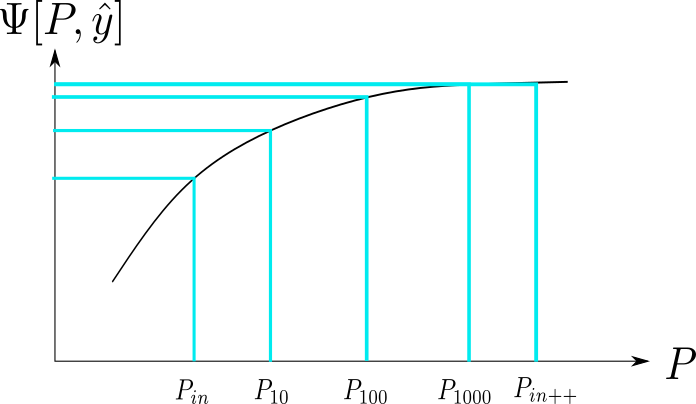
\includegraphics[width=3.5in]
{targeted-est/targeted-p-psi-plot.png}
\caption{
Plot of $\Psi[P, \haty]\in \RR$ versus $P$
at fixed $\haty$.
In reality, the $P$ are not real numbers but
functions.
}
\label{fig-targeted-p-psi-plot.png}
\end{figure}


\section{Functional Calculus}

Define
the Hilbert space of square integrable functions over $\rvX\in S_\rvX$
by

\beq
\calh_\rvX =\{h: (h:S_\rvX\rarrow \RR) \text{ and }
\sum_{ X\in S_ \rvX}[h(X)]^2 <\infty\}
\eeq
For any $f,g\in \calh_\rvX$,
define the dot product (a.k.a. inner product)
of $f$ and $g$ by

\beq
f\cdot g = \sum_X f(X) g(X)
\eeq


Suppose $P:S_\rvX\rarrow [0,1]$
is a probability distribution.
Note that $P\in\calh_\rvX$.
For any $f,g\in\calh_\rvX$,
define the $P$ expected value by

\beq
\av{f}_P = P\cdot f
\eeq
and the $P$ covariance by
\beq
\av{f,g}_P =
\av{fg}_P - \av{f}_P\av{g}_P
\eeq

Suppose $\Psi:\calh_\rvX\rarrow \RR$.
Define the
{\bf functional derivative or gradient }\footnote{
Functional derivatives are commonly used in Physics
especially in Quantum Field Theory.
See Ref.\cite{wiki-func-deri} for more
information about them.}
of $\Psi[\eta]$ with respect to $\eta\in\calh_\rvX$, as follows


\beq
\frac{\delta \Psi[\eta]}
{\delta \eta(a)}=
\lim_{\eps\rarrow 0}
\frac{\Psi[\eta(x)+\eps\frac{\delta(x,a)}{\Delta x}] - \Psi[\eta(x)]}
{\eps}
\eeq
where $\delta(x,a)$ is the Kronecker delta function.
For example,
\beq
\frac{\delta}
{\delta \eta(a)}
\sum_x \Delta x\; \eta(x) h(x)
=
\sum_x \Delta x \frac{\delta(y,a)}{\Delta x} h(x)
=
h(a)
\eeq
 Let
$\delta(x-a)$ denote the Dirac delta function. If we replace
$\frac{\delta(x,a)}{\Delta x}\rarrow\delta(x-a)$
and $\sum_x \Delta x\rarrow \int dx$, we go
from the discrete to the continuous version
of the functional derivative.
In this chapter, we will use only the discrete version.
The $\Delta x$ in the numerator
and the one in the denominator, always cancel out
when we integrate over a Dirac delta function, so we will
henceforth set
$\Delta x=1$.

Suppose $\eta, \eta_0\in \calh_\rvX$. Define the
{\bf functional Taylor expansion} of $\Psi[\eta]$
at $\eta_0$, as follows:

\beq
\Psi[\eta]=
\Psi[\eta_0]
+ \sum_x
\left[
\frac{\delta \Psi[\eta]}
{\delta \eta(x)}\right]_{\eta=\eta_0}
\delta\eta(x)
+
\frac{1}{2!}
\sum_{x,x'}
\left[
\frac{\delta^2 \Psi[\eta]}
{\delta\eta(x)\delta\eta(x') }\right]_{\eta=\eta_0}
\delta\eta(x)\delta\eta(x')
+
\cdots
\eeq
where we abbreviate
$ \eta =\eta(x)$,
$\eta_0=\eta_0(x)$ and $\delta \eta(x) = \eta(x)-\eta_0(x)$.



Define the
{\bf functional directional derivative of $\Psi[\eta]$ in
the $h\in \calh_\rvX$
direction}
by $h\cdot\frac{\delta \Psi[\eta]}{\delta \eta}$.
If one compares functional calculus with vector calculus, we see that
$\frac{\delta \Psi[\eta]}{\delta \eta}$ corresponds to a gradient
$\nabla f(\vecx)$ and
$h\cdot \frac{\delta \Psi[\eta]}{\delta \eta}$
corresponds to a directional derivative
$\vecd\cdot \nabla f(\vecx)$.
For $|\vecd|<<1$, $\vecd\cdot \nabla f(\vecx)$ approximates
the change
in $f(\vecx)$ when $\vecx$ moves from $\vecx$ to $\vecx+\vecd$

Next consider probability
distributions $P, P_{in}:S_\rvX\rarrow [0,1]$
and let

\beq
\cald[\Psi](X)=
\frac{\delta \Psi[P]}
{\delta P(X)}
\;.
\eeq
The linear approximation
to the Taylor expansion of $\Psi[P]$ at
$P_{in}$ is given by

\beq
\underbrace{\Psi[P] - \Psi[P_{in}]}_{\delta \Psi[P,P_{in}]}]=
\sum_X
\underbrace{\left[\frac{\delta\Psi[P]}{\delta P(X)}
\right]_{P=P_{in}}
}_{\cald[P_{in}](X)}
\
\underbrace{\delta P(X)}_{P(X)-P_{in}(X)}
+
\calr[P, P_{in}]
\label{eq-1st-order-psi}
\eeq
If we set

\beq
\cald_{in} = \av{\cald[P_{in}]}_{P_{in}}=\caln(!X)\in\RR
\eeq
and

\beq
\Delta\cald[P](X)= \cald[P](X) - \cald_{in}
\;,
\eeq
then Eq.(\ref{eq-1st-order-psi}) becomes

\beqa
\delta\Psi[P,P_{in}]&=&
\av{\cald[P_{in}]}_P - \cald_{in}
+
\calr[P, P_{in}]
\\
&=&
\av{\Delta\cald[P_{in}]}_P
+
\calr[P, P_{in}]
\eeqa





\section{ATE}

If we set

\beq
\caly_{|d,w}[P] = \sum_y y P(y|d,w) = P(\rvy=1|d,w)
\eeq
and

\beq
\caly_{|d}[P] = \sum_w \caly_{|d,w}[P]P(w)
\;,
\eeq
then the {\bf Average Treatment Effect (ATE)}
is defined as follows

\beq
ATE=\caly_{|1}[P_N]-\caly_{|0}[P_N]
\eeq
The rest of this
chapter is devoted
to discussing ATE estimators.

In discussing ATE,
it is convenient to define the
{\bf propensity}:

\beq
g[P](y) = P(\rvd=1|y)
\eeq
and the
Kronecker difference function
for $d\in \bool$:

\beqa
\Delta(d)&=&
\delta(d, 1)-\delta(d, 0)
\\
&=&
(2d-1)\indi(d\in \bool)
\;.
\eeqa

\begin{claim}
\beq
\av{y \frac{\delta(d',d)}{P(d|w)}}_P
=\caly_{|d'}[P]
\eeq

\end{claim}
\proof
\beqa
\av{y \frac{\delta(d',d)}{P(d|w)}}_P
&=&
\sum_d
\sum_y
\sum_w P(y|d,w)\cancel{P(d|w)}P(w) y \frac{\delta(d',d)}{\cancel{P(d|w)}}
\\
&=&
\sum_y
\sum_w P(y|\rvd=d',w)P(w) y
\\
&=&
\caly_{|\rvd=d'}[P]
\eeqa
\qed

\section{ATE estimators}
\subsection{$\Psi^{G}$}

{\bf General (G) estimator} $\Psi^G$
(a.k.a., G-computation estimator).

\beq
P_N(y,d,w)= \frac{1}{N}\sum_\s \delta(y, y^\s)
\delta(d, d^\s)
\delta(w, w^\s)
\eeq

\beq
P_N(d,w)= \frac{1}{N}\sum_\s \delta(d, d^\s)
\delta(w, w^\s)
\eeq

\beq
P_N(w)= \frac{1}{N}\sum_\s
\delta(w, w^\s)
\eeq

\beq
P_N(y|d,w)= \frac{P_N(y,d,w)}{P_N(d,w)}
\eeq


\beq
\Psi^{G}=\sum_d \sum_w P_N(y|d,w)P_N(w)y\Delta(d)
\eeq


\subsection{$\Psi^{IPW}$}

{\bf Inverse Propensity Weighted (IPW) estimator} $\Psi^{IPW}$
(a.k.a. Inverse Probability of Treatment Weighted (IPTW) estimator).

Assume propensity $P(\rvd=1|w)$ is known.

Define

\beqa
\Psi^{IPW}[P]
&=&
\av{y \frac{\Delta(d)}{P(d|w)}}_P
\eeqa

\beq
\Psi^{IPW}=\Psi^{IPW}[P_N]=
\av{y\frac{\Delta(d)}{P(d|w)}}_{P_N}=
\frac{1}{N}\sum_\s
y^\s \frac{\Delta(d^\s)}{P(d^\s|w^\s)}
\eeq


\subsection{$\Psi^{LIPW}$}

{\bf Linearized IPW (LIPW) estimator} $\Psi^{LIPW}$.


$\Psi^{LIPW}$ is the
{\bf linear approximation (a.k.a.
one-step-approximation)}  of $\Psi^{IPW}[P_{in}]$
in the direction $P_N$.

\beq
\Psi^{IPW}=
\Psi^{IPW}[P_{in}] +
\underbrace{\av{\Delta\cald^{IPW}[P_{in}]}_{P_N}}
_{P_N\cdot\Delta\cald^{IPW}[P_{in}]}
\eeq


\begin{claim}
\label{cl-grad-ipw}
\beq
\cald^{IPW}[P](X) =  \caly_{|1,w}[P]
-
\caly_{|0,w}[P]
+
\frac{\Delta(d)}{P(d|w)}
(y-\caly_{|d,w}[P])
\eeq
\end{claim}
\proof
\beqa
\frac{\delta \Psi^{IPW}[P]}
{\delta P(X)}
&=&
\sum_{X'} y' \Delta(d')\frac{\delta}{\delta P(X)}
\frac{P(X')}{P(d'|w')}
\eeqa

\beqa
\frac{\delta}{\delta P(X)}
\frac{P(X')}{P(d'|w')}
&=&
\frac{\delta(X,X')}{P(d'|w')}
-\frac{P(X')}{[P(d'|w')]^2}
\frac{\delta P(d'|w')}{\delta P(X)}
\\
&=&
\frac{\delta(X, X')}{P(d'|w')}
-\frac{P(X')}{P(d'|w')}
\frac{\delta \ln P(d'|w')}{\delta P(X)}
\\
&=&
\underbrace{\frac{\delta(X, X')}{P(d'|w')}}_{\delta^3/P(d'|w')}
-P(y'|d',w')P(w')
\frac{\delta \ln P(d'|w')}{\delta P(X)}
\eeqa

\beqa
\frac{\delta \ln P(d',w')}{\delta P(X)}
&=&
\frac{1}{P(d',w')}
\sum_{y'}\frac{\delta P(X')}{\delta P(X)}
\\
&=&
\underbrace{\frac{\delta(d, d')\delta(w,w')}{P(d',w')}}_{\delta^2/P(d',w')}
\eeqa

\beqa
\frac{\delta \ln P(w')}{\delta P(X)}
&=&
\underbrace{\frac{\delta(w,w')}{P(w')}}_{\delta^1/P(w')}
\eeqa

\beqa
\frac{\delta \ln P(d'|w')}{\delta P(X)}
&=&
\frac{\delta^2}{P(d',w')}
-
\frac{\delta^1}{P(w')}
\eeqa

\beq
\frac{\delta}{\delta P(X)}
\frac{P(X')}{P(d'|w')}
=
\frac{\delta^3}{P(d'|w')}
-P(y'|d',w')P(w')
\left[
\frac{\delta^2}{P(d',w')}
-
\frac{\delta^1}{P(w')}
\right]
\eeq

\beq
\sum_{X'} y'\Delta(d')\left[
\frac{\delta^3}{P(d'|w')}
\right]
=\boxed{\frac{\Delta(d)}{P(d|w)}y}
\eeq

\begin{align}
\sum_{X'} y'\Delta(d')
\left[
\frac{-P(y'|d',w')\delta^2}{P(d'|w')}
\right]
&=
-\sum_{y'}
y'\Delta(d)
\frac{P(y'|d,w)}{P(d|w)}
\\
&=
\boxed{\frac{\Delta(d)}{P(d|w)}
(-\caly_{|d,w}[P])}
\end{align}

\beqa
\sum_{X'} y'\Delta(d')
\left[P(y'|d',w')\delta^1
\right]
&=&
\sum_{y'}\sum_{d'} y'\Delta(d')
P(y'|d',w)
\\
&=&
\boxed{\caly_{|1,w}[P]-\caly_{|0,w}[P]}
\eeqa
\qed

\begin{claim}
\beq
\av{\cald^{IPW}[P]}_P=\Psi^{IPW}[P]
\eeq
Hence,

\beq
\cald^{IPW}_{in}=\av{\cald^{IPW}[P_{in}]}_{P_{in}}=\Psi^{IPW}[P_{in}]
\eeq

\end{claim}
\proof

\beq
\cald^{IPW}[P](X) =  \caly_{|1,w}[P]
-
\caly_{|0,w}[P]
+
\frac{\Delta(d)}{P(d|w)}
(y-\caly_{|d,w}[P])
\eeq

\beqa
\av{\caly_{|1,w}[P]-\caly_{|0,w}[P]}_P
&=&
\sum_w P(w)(\caly_{|1,w}[P]-\caly_{|0,w}[P])
\\
&=&
\Psi^{IPW}[P]
\eeqa

\beq
\av{\frac{\Delta(d)}{P(d|w)}y}_P
=
\Psi^{IPW}[P]
\eeq

\beqa
\av{\frac{\Delta(d)}{P(d|w)}
\caly_{|d,w}[P]}_P
&=&
\sum_y\sum_w \sum_d
 P(y|d,w)P(w)\Delta(d)\caly_{|d,w}[P]
 \\
 &=&
\sum_w \sum_d
 P(w)\Delta(d)\caly_{|d,w}[P]
 \\
 &=&
\Psi^{IPW}[P]
\eeqa
\qed

Note the following cancellation:
\beqa
\Psi^{IPW}[P] &=&
\Psi^{IPW}[P_{in}]
 + \av{\cald^{IPW}[P_{in}]}_P -\cald^{IPW}_{in}
 + \calr^{IPW}[P,P_{in}]
\\
&=&
\cancel{\Psi^{IPW}[P_{in}] }
 + \av{\cald^{IPW}[P_{in}]}_P -\cancel{\Psi^{IPW}[P_{in}] }
 + \calr^{IPW}[P,P_{in}]
 \\
&=&
 \av{\cald^{IPW}[P_{in}]}_P
 + \calr^{IPW}[P,P_{in}]
\eeqa

\begin{claim}
\label{cl-remainder-taylor-exp}
\begin{align}
\calr^{IPW}[P,P_{in}]&=-
\sum_w P(w)\sum_d \Delta(d)
\left(
P(d|w)-P_{in}(d|w)
\right)
\left(
\frac{
\caly_{|d,w}[P]-\caly_{|d,w}[P_{in}]}
{P_{in}(d|w)}
\right)
\end{align}
\end{claim}
\proof

\begin{align}
\calr^{IPW}[P,P_{in}]
&=
\Psi^{IPW}[P]
-\av{\cald^{IPW}[P_{in}]}_P
\\
&=
\av{
y \frac{\Delta(d)}{P(d|w)}
-
\left(
\caly_{|1,w}[P_{in}]
-
\caly_{|0,w}[P_{in}]
+
\frac{\Delta(d)}{P_{in}(d|w)}
(y-\caly_{|d,w}[P_{in}])
\right)
}_{P}
\\
&=
\left\{
\begin{array}{l}
\sum_w P(w)\left(
-\caly_{|1,w}[P_{in}]
+
\caly_{|0,w}[P_{in}]
\right)
\\
+\sum_{d,w} P(d,w) \left(
\frac{\Delta(d)}{P_{in}(d|w)}
\caly_{|d,w}[P_{in}]
\right)
\\
+\sum_{y,d,w} P(y, d,w)\left(
\frac{1}{P(d|w)}- \frac{1}{P_{in}(d|w)}
\right) y\Delta(d)
\end{array}
\right.
\\
&=\sum_w P(w)\sum_d \Delta(d)
\left\{
\begin{array}{l}
\left(
\frac{P(d|w)}{P_{in}(d|w)}-1
\right)
\caly_{|d,w}[P_{in}]
\\
+\sum_{y}P(y|d,w)\left(
\frac{P_{in}(d|w)-P(d|w)}{P_{in}(d|w)}
\right) y
\end{array}
\right.
\\
&=
\sum_w P(w)\sum_d \Delta(d)
\left(\frac{P(d|w)}{P_{in}(d|w)}-1
\right)
(\caly_{|d,w}[P_{in}]-
\caly_{|d,w}[P])
\end{align}

\qed

Claim \ref{cl-remainder-taylor-exp}
allows us to put a bound
on the absolute value of the remainder $\calr^{IPW}$:

\begin{align}
|\calr^{IPW}[P,P_{in}]|&\leq
\sum_d \sum_w
\underbrace{\sqrt{P(w)}
\left|
P(d|w)-P_{in}(d|w)
\right|}_{A(d,w)}
\underbrace{\sqrt{P(w)}
\left|
\frac{
\caly_{|d,w}[P]-\caly_{|d,w}[P_{in}]}
{P_{in}(d|w)}
\right|}_{B(d,w)}
\nonumber
\\&
\quad\text{(because
$|\Delta(d)|\leq 1$, and $\left|\sum_i a_i\right|\leq \sum_i |a_i|$ )}
\\
&\leq
\sum_d
\underbrace{\sqrt{\sum_w A^2(d,w)}}_{A(d)}
\underbrace{\sqrt{\sum_w B^2(d,w)}}_{B(d)}
\quad \text{(because $\veca\cdot \vecb\leq |\veca|\;|\vecb|$)}
\end{align}

\beqa
A(d')&=&
\sum_w P(w)
\left(
P(d'|w)-P_{in}(d'|w)
\right)^2
\\
&=&
\av{
\left(
P(d'|w)-P_{in}(d'|w)
\right)^2
}_P
\eeqa

\beqa
B(d')&=&
\sum_w P(w)
\left(
\frac{
\caly_{|d',w}[P]-\caly_{|d',w}[P_{in}]}
{P_{in}(d'|w)}
\right)^2
\\
&=&
\av{
\left(
\frac{
\caly_{|d',w}[P]-\caly_{|d',w}[P_{in}]}
{P_{in}(d'|w)}
\right)^2
}_P
\eeqa

\begin{align}
|\calr^{LIPW}[P_N,P_{in}]|&\leq
\sum_{d'=0}^1
\underbrace{
\av{
\left(
P_N(d'|w)-P_{in}(d'|w)
\right)^2
}_{P_N}
}_{A_N(d')}
\underbrace{
\av{
\left(
\frac{
\caly_{|d',w}[P_N]-\caly_{|d',w}[P_{in}]}
{P_{in}(d'|w)}
\right)^2
}_{P_N}
}_{B_N(d')}
\end{align}

If either $A_N(1)=A_N(0)=0$ (i.e.,
zero error in the propensities) or $B_N(0)=B_N(1)=0$ (i.e.,
zero bias),
then $\calr^{LIPW}[P_N,P_{in}]=0$.
This property
of $\Psi^{LIPW}$ is referred to as {\bf double robustness}.


\subsection{$\Psi^{LIPW++}$ (a.k.a $\Psi^{TMLE}$)}

{\bf Substitutional LIPW (LIPW++) estimator}
(a.k.a, targeted minimum loss estimator (TMLE)) $\Psi^{LIPW++}$.

$\Psi^{LIPW++}$ is the
linear approximation
 of $\Psi^{IPW}[P_{in}]$ at the point $P_{in}=P_{in++}$,
in the direction $P_N$,
where the slope
of loss function at $P_{in}=P_{in++}$ is zero

\beq
\Psi^{LIPW++}=\Psi^{TMLE}=
\Psi^{IPW}[P_{in++}] +
\underbrace{\av{\Delta\cald^{IPW}[P_{in++}]}_{P_N}}_{=0}
\eeq

$P_N\cdot \Delta\cald^{IPW}[P_{in++}]=0$
means $P_N$ (for all $N$)
points perpendicular to the
gradient of $\Delta\Psi^{IPW}[P]$
evaluated at $P=P_{in++}$.
(gradients point in the direction
of maximum change).
This property of
of $\Psi^{TMLE}$ is referred to as {\bf substitution
invariance}, and $\Psi^{TMLE}$
is said to be a {\bf substitution estimator}.
A substitution estimator is
very desirable because
its
absolute value is bounded, unlike
the value of $\Psi^{LIPW}$.

$\Psi^{TMLE}$ is both
a doubly robust estimator and a substitution estimator.

Claim \ref{cl-grad-ipw} allows us
express
more explicitly the constraint that defines $P_{in++}$:

\begin{align}
0 &=
P_N\cdot\Delta\cald^{IPW}[P_{in++}]
\\
0 &=-\cald^{LPW}_{in}[P_{in++}]+
P_N\cdot\cald^{IPW}[P_{in++}]
\\
&= -\cald^{LPW}_{in}[P_{in++}]+
\left\{
\begin{array}{l}
\overbrace{
\frac{1}{N}
\sum_\s
\left(
\caly_{|1,w^\s}[P_{in++}]
-
\caly_{|0,w^\s}[P_{in++}]
\right)
}^{ \cald^{LPW}_{in}[P_{in++}]}
\\
+
\frac{1}{N}
\sum_\s
\frac{\Delta(d^\s)}{P_{in++}(d^\s|w^\s)}
(y^\s-\caly_{|d^\s,w^\s}[P_{in++}])
\end{array}
\right.
\\
&=
\frac{1}{N}
\sum_\s
\frac{\Delta(d^\s)}{P_{in++}(d^\s|w^\s)}
(y^\s-\caly_{|d^\s,w^\s}[P_{in++}])
\end{align}


\begin{figure}[h!]
\centering
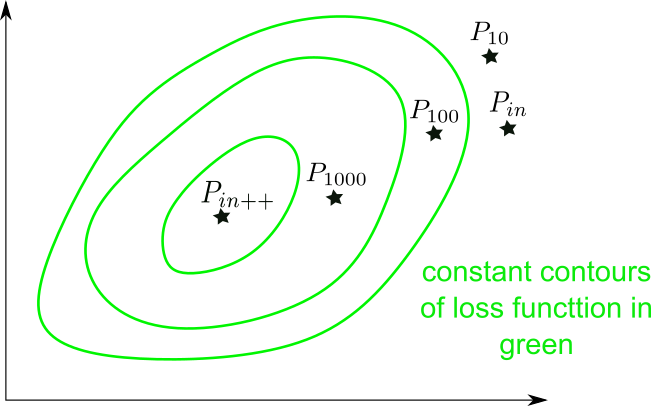
\includegraphics[width=3.5in]
{targeted-est/targeted-est.png}
\caption{
This figure portrays
the space of functions $\calh_\rvX$
as if it were the real plane $\RR^2$,
and the functional $\Psi^{IPW}:\calh_\rvX\rarrow\RR$
as if it were a real valued function on $\RR^2$.
It shows  the constant contours
of the loss function $\call$ in green.
$P_N$ for $N=100, 200, 300$
represent empirical distributions.
The gradient of $\call$
is perpendicular to $P_N$  at $P_{in++}$
but not at $P_{in}$.
}
\label{fig-targeted-est}
\end{figure}

Use as loss function $\call$ the Cross Entropy
$CE(p\parallel q)$ for $p, q\in [0,1]$
\beq
\call = CE(p\parallel q)=-[p \ln q + (1-p) \ln(1- q)]
\eeq
$\call\geq 0$ and is minimum when $p=q$.
When $p=q$, it equals the entropy of $p$,
i.e., when $p=q$, $\call=-\sum_{x\in \bool} P(x)\ln P(x)= H(P)$,
where $P(0)=p, P(1)=1-p$.

For some $y\in\bool$ and $\eps>0$,
set\footnote{To agree with the TE literature,
we are using $\expit(x)$
(resp., $\logit(p)$) to denote
the sigmoid function (resp., log-odds function)
which we normally
denote in this book by
 $\smoid(x)$ (resp., $\lodds(p)$).}

\beq
p=y,
\quad
q= \expit[\logit(q_0) + \eps \beta ]
\eeq
in the loss function $\call$
and call it $\call=\call(\beta, y, q_0, \eps)$.
Note that since $q=y$ is binary,
the minimum of this loss function is zero.

 Recall that in Section \nameref{sec-smoid}, we proved that
 the derivative of $\expit(x)$ satisfies

\beq
\expit'(x) = \expit(x)[1-\expit(x)]
\;.
\eeq
Hence,

\begin{align}
\lim_{\eps\rarrow 0}\partial_\eps \call(\beta, y, q_0, \eps)
&=
\lim_{\eps\rarrow 0}
\left[-\frac{p}{q} + \frac{1-p}{1-q}\right]\partial_\eps q
\\
&=
\left[-\frac{y}{q_0} + \frac{1-y}{1-q_0}\right]
\lim_{\eps\rarrow 0}
\left\{
\begin{array}{l}
\expit[\logit(q_0) + \eps \beta ]
\\
*\left\{1-\expit[\logit(q_0) + \eps \beta ]\right\}
\beta
\end{array}
\right.
\\
&=
\left[-\frac{y}{q_0} + \frac{1-y}{1-q_0}\right]
q_0(1-q_0)\beta
\\
&=
\beta[q_0-y]
\end{align}

If we define $\cald^\s$ by

\beq
\cald^\s = \lim_{\eps\rarrow 0}\partial_\eps\call
\left(
\begin{array}{l}
\beta=\frac{\Delta(d^\s)}{P_{in++}(d^\s|w^\s)} ,
\\
y=y^\s,
\\
q_0 = \caly_{|d^\s,w^\s}[P_{in++}],
\\
\eps =\eps
\end{array}
\right)
\;,
\eeq
then

\beq
\frac{1}{N}\sum_\s\cald^\s =P_N\cdot \cald= 0
\;.
\eeq

It is also possible
to express $\cald^\s$
as a functional gradient instead
of an $\eps\rarrow 0$ limit.
Indeed, note that


\beq
\cald^\s = \frac{\delta}{\delta h(X^\s)}
\left(
\begin{array}{l}
\beta=\sum_{X}h(X)\frac{\Delta(d)}{P_{in++}(d|w)} ,
\\
y=y^\s,
\\
q_0 = \caly_{|d^\s,w^\s}[P_{in++}],
\\
\eps =1
\end{array}
\right)
\eeq

\beq
\frac{1}{N}\sum_\s\frac{\delta\call}{\delta h(X^\s)}
=P_N\cdot \frac{\delta\call}{\delta h}= 0
\eeq

An approximation commonly made
at this point is to assume that $h(X)$ has
the special form:

\beq
h(X) = \gamma\delta(X,\hat{X})
\eeq
for some $\gamma\in \RR$. When
this is the case,

\beq
\beta = \gamma\frac{\Delta(\hat{d})}{P_{in++}(\hat{d}|\hat{w})}
\eeq

\section{$\Psi^{TMLE}$ in practice}
